\documentclass{beamer}
\usepackage[english, russian]{babel}
\usepackage[T2A]{fontenc}
\usepackage[utf8]{inputenc}
\usepackage{indentfirst}
\usepackage{amsmath, amsfonts, amssymb, amsthm, mathtools}
\usepackage[export]{adjustbox}
\usepackage{graphicx} 
\graphicspath{ {./images/} }

\usepackage{subcaption}
\usepackage{verbatim}

\usepackage{minted}{\setlength{\parskip}{0pt}}

\usepackage{hyperref}

\hypersetup{
    colorlinks=true,
    linkcolor=blue,
    filecolor=magenta,      
    urlcolor=black,
    pdftitle={Overleaf Example},
    pdfpagemode=FullScreen,
    }


\title{Лабораторная работа № 2. \\ Настройка DNS-сервера.}
\author{Данила Стариков \\ НПИбд-02-22}
\institute{Российский университет дружбы народов имени Патриса Лумумбы}
\date{2024}

\begin{document}

\frame{\titlepage}

\begin{frame}
\frametitle{Цель работы}
\begin{itemize}
    \item Приобретение практических навыков по установке и конфигурированию DNS-сервера, усвоение принципов работы системы доменных имён.
\end{itemize}
\end{frame}

\begin{frame}
\frametitle{Установка DNS-сервера}
    \centering
    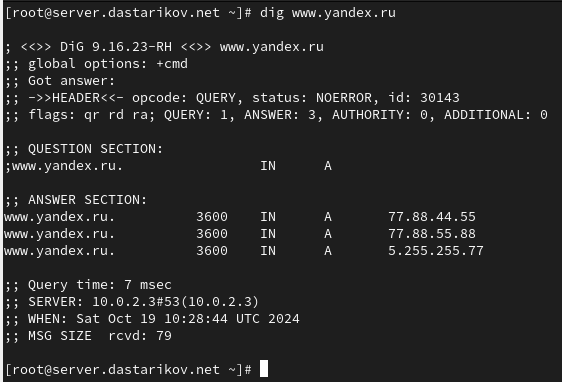
\includegraphics[width=0.8\textwidth]{../images/image01.png}
    \captionof{figure}{Запрос к DNS-адресу www.yandex.ru}
\end{frame}

\begin{frame}
\frametitle{Конфигурирование кэширующего DNS-сервера при отсутствии фильтрации DNS-запросов маршрутизаторами}
    \centering
    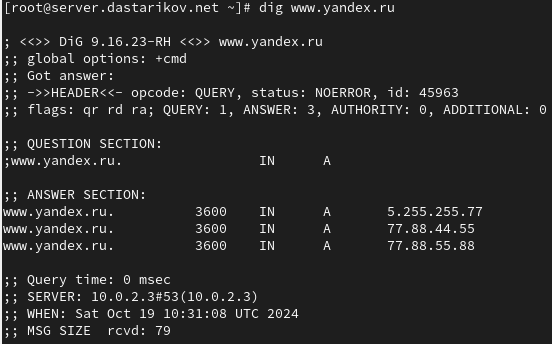
\includegraphics[width=0.8\textwidth]{../images/image02.png}
    \captionof{figure}{Запрос к DNS-адресу www.yandex.ru}
\end{frame}


\begin{frame}
\frametitle{Конфигурирование кэширующего DNS-сервера при отсутствии фильтрации DNS-запросов маршрутизаторами}
    \centering
    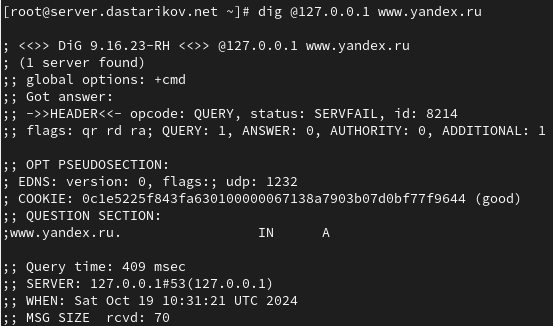
\includegraphics[width=0.8\textwidth]{../images/image03.png}
    \captionof{figure}{Запрос к DNS-адресу www.yandex.ru с заданным адресом сервера.}
\end{frame}


\begin{frame}
\frametitle{Конфигурирование кэширующего DNS-сервера при отсутствии фильтрации DNS-запросов маршрутизаторами}
    \centering
    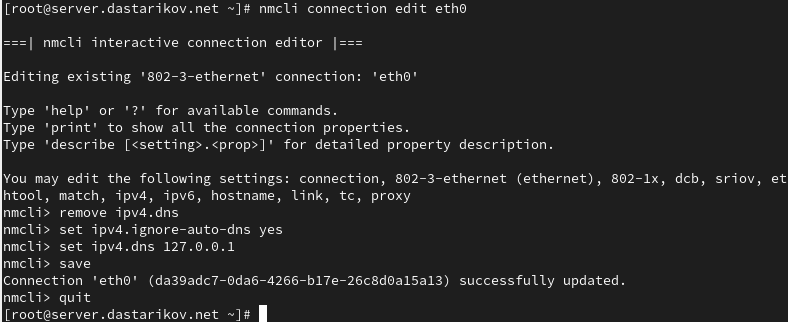
\includegraphics[width=0.8\textwidth]{../images/image04.png}
    \captionof{figure}{Настройка сетевого соединения eth0.}
\end{frame}


\begin{frame}
\frametitle{Конфигурирование кэширующего DNS-сервера при отсутствии фильтрации DNS-запросов маршрутизаторами}
    \centering
    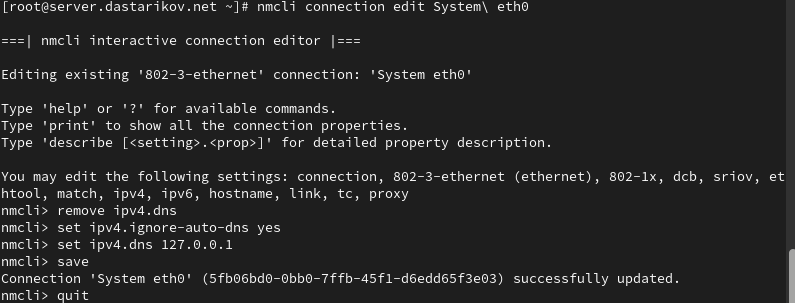
\includegraphics[width=0.8\textwidth]{../images/image05.png}
    \captionof{figure}{Настройка сетевого соединения System eth0.}
\end{frame}


\begin{frame}
\frametitle{Конфигурирование кэширующего DNS-сервера при отсутствии фильтрации DNS-запросов маршрутизаторами}
    \centering
    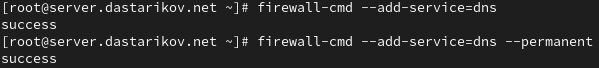
\includegraphics[width=0.8\textwidth]{../images/image06.png}
    \captionof{figure}{Настройка межсетевого экрана.}
\end{frame}


\begin{frame}
\frametitle{Конфигурирование кэширующего DNS-сервера при отсутствии фильтрации DNS-запросов маршрутизаторами}
    \centering
    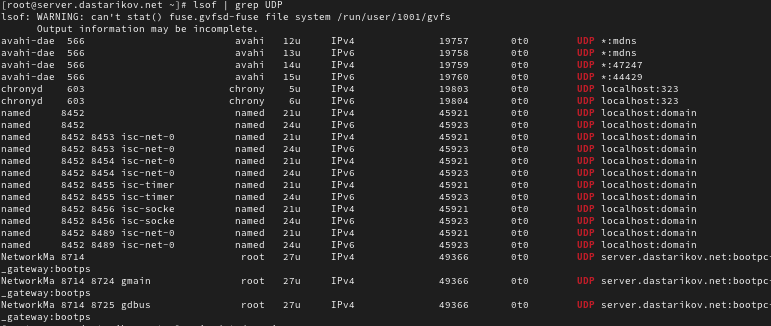
\includegraphics[width=0.8\textwidth]{../images/image07.png}
    \captionof{figure}{Просмотр прослушиваемых портов.}
\end{frame}


\begin{frame}
\frametitle{Конфигурирование кэширующего DNS-сервера при наличии фильтрации DNS-запросов маршрутизаторами}
    \centering
    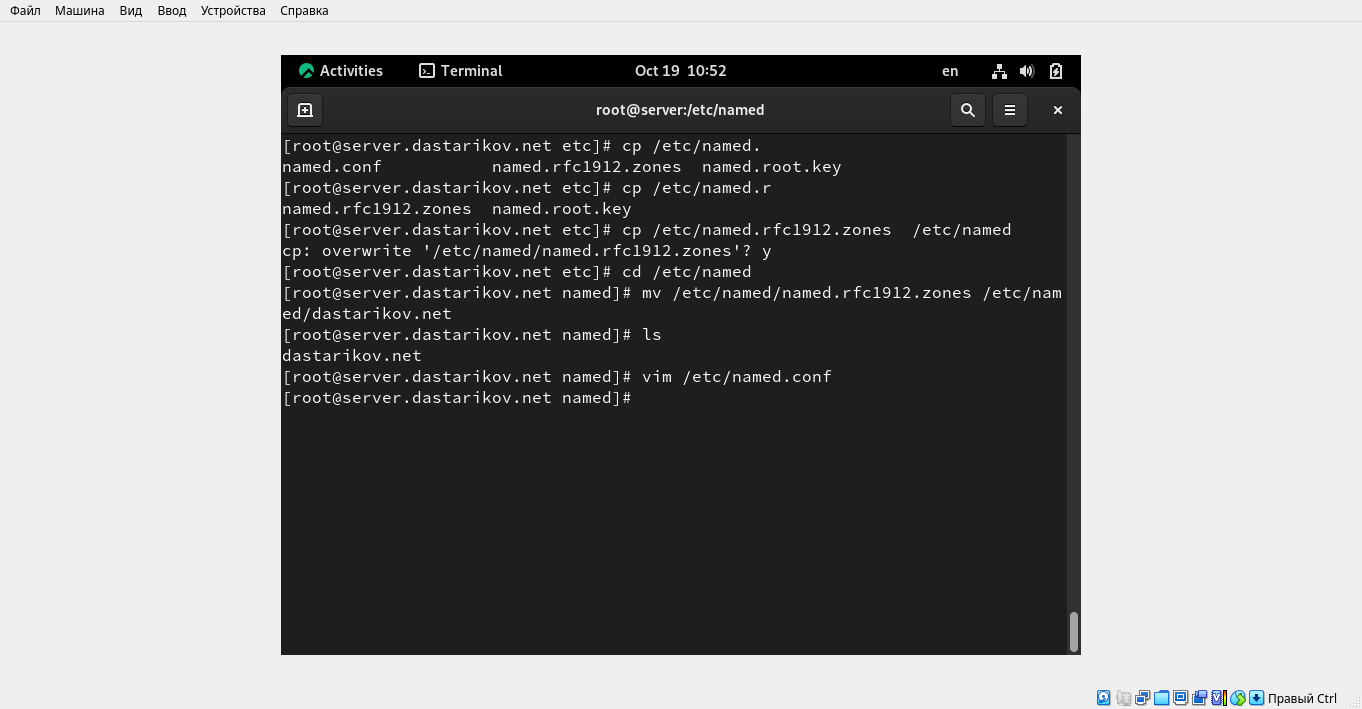
\includegraphics[width=0.8\textwidth]{../images/image08.png}
    \captionof{figure}{Настройка файлов для описания DNS-зон.}
\end{frame}


\begin{frame}
\frametitle{Конфигурирование кэширующего DNS-сервера при наличии фильтрации DNS-запросов маршрутизаторами}
    \centering
    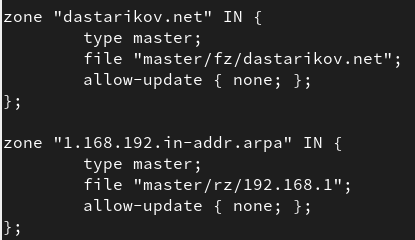
\includegraphics[width=0.8\textwidth]{../images/image09.png}
    \captionof{figure}{Описание DNS-зон.}
\end{frame}


\begin{frame}
\frametitle{Конфигурирование кэширующего DNS-сервера при наличии фильтрации DNS-запросов маршрутизаторами}
    \centering
    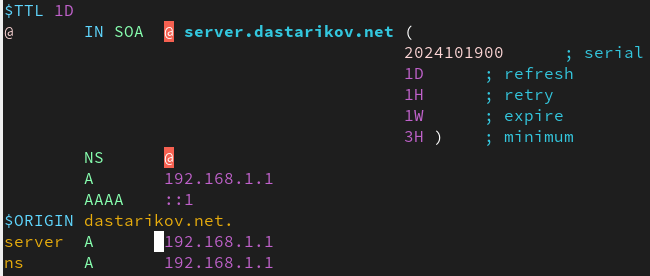
\includegraphics[width=0.8\textwidth]{../images/image10.png}
    \captionof{figure}{Настройка прямой DNS-зоны.}
\end{frame}


\begin{frame}
\frametitle{Конфигурирование кэширующего DNS-сервера при наличии фильтрации DNS-запросов маршрутизаторами}
    \centering
    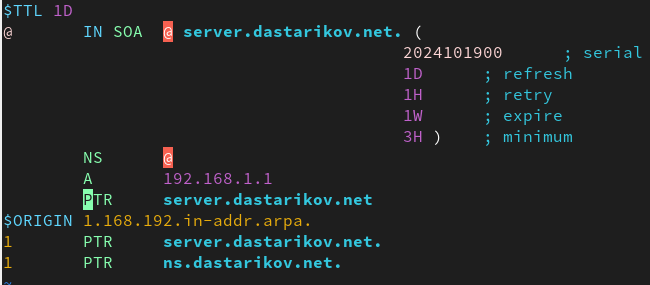
\includegraphics[width=0.8\textwidth]{../images/image11.png}
    \captionof{figure}{Настройка обратной DNS-зоны.}
\end{frame}


\begin{frame}
\frametitle{Конфигурирование кэширующего DNS-сервера при наличии фильтрации DNS-запросов маршрутизаторами}
    \centering
    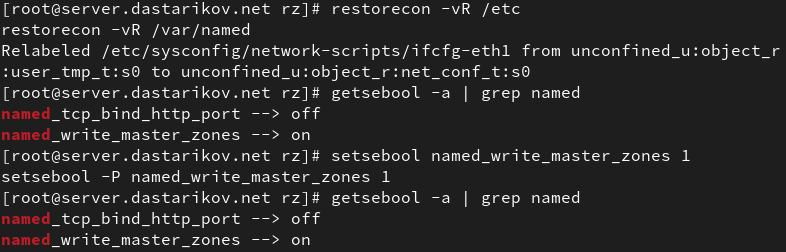
\includegraphics[width=0.8\textwidth]{../images/image12.png}
    \captionof{figure}{Настройка меток SELinux.}
\end{frame}


\begin{frame}
\frametitle{Конфигурирование кэширующего DNS-сервера при наличии фильтрации DNS-запросов маршрутизаторами}
    \centering
    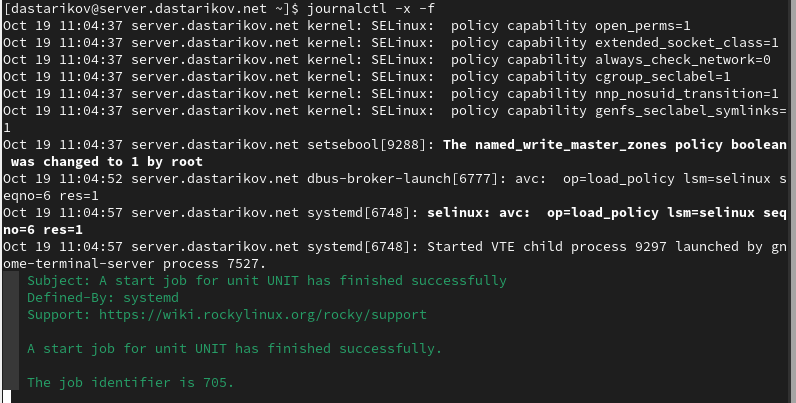
\includegraphics[width=0.8\textwidth]{../images/image13.png}
    \captionof{figure}{Просмотр записей журнала системных сообщений.}
\end{frame}


\begin{frame}
\frametitle{Анализ работы DNS-сервера}
    \centering
    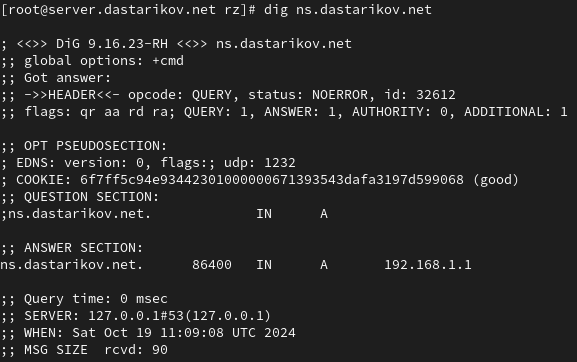
\includegraphics[width=0.8\textwidth]{../images/image14.png}
    \captionof{figure}{Получение описания DNS-зоны с сервара.}
\end{frame}

\begin{frame}
\frametitle{Анализ работы DNS-сервера}
    \centering
    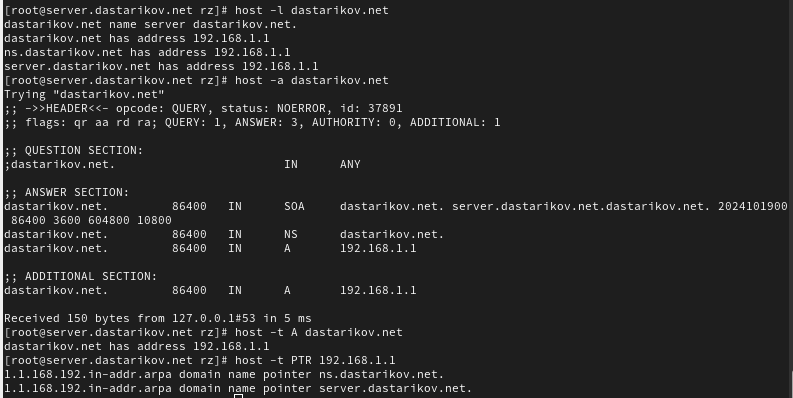
\includegraphics[width=0.8\textwidth]{../images/image16.png}
    \captionof{figure}{Проверка корректиности работы DNS-сервера.}
\end{frame}



\begin{frame}
\frametitle{Выводы}
\begin{itemize}
    \item В результате лабораторной работы приобрели практические навыки по установке и конфигурированию DNS-сервера.
\end{itemize}
\end{frame}
\end{document}
